\chapter{Methodik}

\label{ch:methodik}

In diesem Kapitel werden die Funktionsweisen des algorithmischen und des KI-basierten Ansatzes detailliert beschrieben. Die zugrunde liegende Bildverarbeitungspipeline ist in Abbildung \ref{fig:algo_pipe} dargestellt und gliedert sich in die folgenden aufeinanderfolgenden Schritte: Vorverarbeitung, Erkennung der Dartscheibe, perspektivische Korrektur, Lokalisierung der Segmentringe, Lokalisierung der Segmentlinien sowie die abschließende Berechnung des Scores. Die Reihenfolge der Schritte ist dabei verbindlich und muss zwingend eingehalten werden.

\begin{figure}[H]
    \centering
    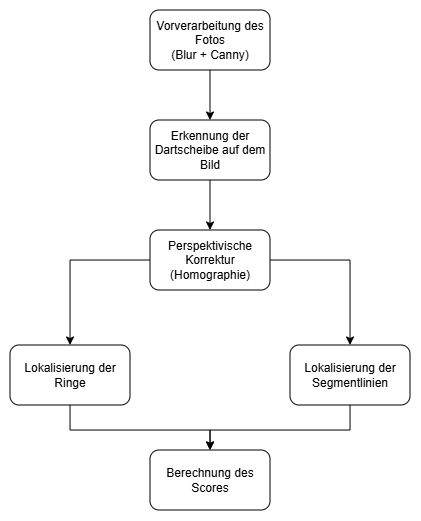
\includegraphics[width=0.5\textwidth]{images/algorithmische_pipeline.png}
    \caption{Übersicht über die algorithmische Pipeline}
    \label{fig:algo_pipe}
\end{figure}

Darüber hinaus werden die Vergleichskriterien beider Ansätze erläutert sowie die Vorgehensweise beim Vergleich beschrieben.

\newpage

\section{Algorithmischer Ansatz}

Der entwickelte algorithmische Ansatz dient der vollständigen Lokalisierung und geometrischen Segmentierung einer Dartscheibe in mobilen Bildaufnahmen ohne den Einsatz lernbasierter Verfahren. Dabei wird vorausgesetzt, dass die Dartscheibe in der Aufnahme näherungsweise frontal erfasst wird und somit als Kreis erscheint. Perspektivisch bedingte Verzerrungen sowie deren Korrektur konnten in diesem Ansatz nicht berücksichtigt werden.

\subsection{Vorverarbeitung}

Als erster Schritt der Pipeline wird das Eingangsfoto, das auf eine Auflösung von 3000 x 4000 Pixeln festgelegt wurde, vorverarbeitet und für die weitere Verarbeitung aufbereitet. Hierzu wird das Bild vom RGB- in das Graustufenformat konvertiert. Zur Reduktion von Bildrauschen kommt ein Median-Filter mit einer Kernelgröße von $k = 11$ zum Einsatz. 

\subsection{Erkennung der Dartscheibe}

Die Lokalisierung der Dartscheibe erfolgt mittels der Hough-Kreiserkennung, die auf dem vorverarbeiteten Graustufenbild operiert. 

Der minimale und maximale Suchradius werden dynamisch in Abhängigkeit der kürzeren Bildkante berechnet. Ausgehend von einem initialen Wertebereich von 70\,\% bis 75\,\% der Bildkantenlänge wird der Suchbereich iterativ um jeweils 5\,\% reduziert, sofern keine Kreishypothese gefunden wurde. Die Methode wird mit einem Kantenschwellwert von $\mathtt{param1} = 300$, einem Akkumulatorschwellwert von $\mathtt{param2} = 200$, einem minimalen Kreismittelabstand von $\mathtt{minDist} = 0{,}8 \cdot h$ -- wobei $h$ die Bildhöhe bezeichnet -- sowie einem inversen Auflösungsverhältnis von $\mathtt{dp} = 1{,}5$ konfiguriert. 

Die Ausgabe des Verfahrens ist ein erkannter Kreis, beschrieben durch Mittelpunkt $(a, b)$ und Radius~$r$, welcher dem Rand der Dartscheibe entspricht.

\section{Machine Learning Ansatz}

\label{sec:ml-ansatz}

\subsection{Erkennung der Dartscheibe}

\subsection{Nachverarbeitung der Maske}

\section{Gemeinsame Verarbeitungsschritte}

Nach erfolgreicher Detektion der Dartscheibe im Bild werden, unabhängig vom jeweils verwendeten Verfahren, identische nachgelagerte Verarbeitungsschritte durchgeführt. Als Voraussetzung für diese weiteren Schritte wird die erkannte Dartscheibe in einer standardisierten geometrischen Form repräsentiert. Im Fall einer kreisförmigen Approximation erfolgt die Beschreibung durch den Mittelpunkt mit den Koordinaten $x$ und $y$ sowie den Radius $r$. Bei einer elliptischen Approximation wird die Dartscheibe durch den Mittelpunkt (x,y), die Längen der Haupt- und Nebenachse (major bzw. minor axis) sowie den Rotationswinkel der Ellipse (angle) beschrieben.

\subsection{Perspektivische Korrektur und Normalisierung}

\label{sec:homography}

Nach der Lokalisierung der Dartscheibe wird das Eingabebild mittels einer Homographie auf ein einheitliches quadratisches Format von $1024 \times 1024$ Pixeln transformiert. Dafür sind mindestens vier Referenzpunkte nötig, die sich abhängig davon berechnen, ob die erkannte Dartscheibe als Kreis oder Ellipse vorliegt.

\textbf{Kreisförmige Spielfläche:} Wird die Dartscheibe als Kreis mit Mittelpunkt $(c_x, c_y)$ und Radius $r$ beschrieben, so werden die vier Quellpunkte als Ecken des umbeschriebenen achsenparallelen Quadrats gewählt:

\begin{equation}
P_1 = \begin{pmatrix} c_x - r \\ c_y - r \end{pmatrix}, \quad
P_2 = \begin{pmatrix} c_x + r \\ c_y - r \end{pmatrix}, \quad
P_3 = \begin{pmatrix} c_x + r \\ c_y + r \end{pmatrix}, \quad
P_4 = \begin{pmatrix} c_x - r \\ c_y + r \end{pmatrix}
\end{equation}

Die Punkte sind symmetrisch um den Mittelpunkt verteilt und spannen ein Quadrat auf, dessen Seitenlänge dem Durchmesser $2r$ des Kreises entspricht.

\textbf{Elliptische Spielfläche:} 

% Liegt die Dartscheibe als Ellipse vor, ist diese durch ihren Mittelpunkt $(c_x, c_y)$, die Hauptachse $MA$, die Nebenachse $ma$ sowie einen Rotationswinkel $\alpha$ definiert. Daraus ergeben sich die Halbachsen $a = MA/2$ und $b = ma/2$. Um die geometrische Ausrichtung der Ellipse zu berücksichtigen, wird der Winkel $\alpha$ in das Bogenmaß $\theta$ umgerechnet und die zugehörige 2D-Rotationsmatrix gebildet:

% \begin{equation}
% R(\theta) = \begin{pmatrix} \cos\theta & -\sin\theta \\ \sin\theta & \cos\theta \end{pmatrix}
% \end{equation}

% In einem lokalen Koordinatensyste, in welchem der Mittelpunkt der Ellipse den Ursprung bildet, können die vier Ecken des umschreibenden Rechtecks folgendermaßen definiert werden:

% \begin{equation}
% \mathbf{p}_1^{\text{lok}} = \begin{pmatrix} -a \\ -b \end{pmatrix}, \quad
% \mathbf{p}_2^{\text{lok}} = \begin{pmatrix}  a \\ -b \end{pmatrix}, \quad
% \mathbf{p}_3^{\text{lok}} = \begin{pmatrix}  a \\  b \end{pmatrix}, \quad
% \mathbf{p}_4^{\text{lok}} = \begin{pmatrix} -a \\  b \end{pmatrix}
% \end{equation}

% Anschließend werden diese Punkte durch die Rotationsmatrix $R(\theta)$ in die Ausrichtung der Ellipse überführt und um den Mittelpunkt $(c_x, c_y)$ in das globale Bildkoordinatensystem verschoben:

% \begin{equation}
% \mathbf{p}_i = R(\theta) \cdot \mathbf{p}_i^{\text{lok}} + \begin{pmatrix} c_x \\ c_y \end{pmatrix},
% \qquad i \in \{1, 2, 3, 4\}
% \end{equation}

% Die so berechneten Punkte beschreiben die Ecken des rotierten, der Ellipse umbeschriebenen Rechtecks im Bildkoordinatensystem. Diese vier Punkte dienen anschließend als Quellpunkte für die Berechnung der Homographiematrix, mit der die perspektivische Verzerrung der Spielfläche korrigiert wird.

% To Do: Ellipsen - Transformation implementieren. Problem: durch die oben beschriebene Normalisierung wird zwar das Rechteck der Ellipse Normalisiert aber nicht der Dartscheibe. Die 20 könnte als irgendwo einfach sein. Idee: Einmal austesten wo die 20 ist und dann einfach die Scheibe weiter drehen.

\subsection{Lokalisierung der Ringe}

Nach der perspektivischen Normalisierung liegt die Dartscheibe als
frontale Draufsicht im einheitlichen $1024 \times 1024$-Format vor.
In diesem Koordinatensystem befindet sich der Scheibenmittelpunkt
näherungsweise bei $(512, 512)$. Die geometrische Struktur einer
Dartscheibe besteht aus konzentrischen Ringen mit definierten Radien,
die auf Basis der normierten Darstellung mittels erneuter
Hough-Kreiserkennung detektiert werden.

Die Implementierung der Hough-Transformation durch die Bibliothek opencv-python enthält einen Parameter \texttt{minDist}. Dieser gibt den minimalen Abstand zwischen zwei erkannten Kreisen in Pixel an. Dies ist für die Erkennung der Ringsegmente einer Dartscheibe problematisch, da sich diese einen Mittelpunkt teilen, wobei sich nur die Radien unterscheiden. Da sich dieser Parameter nicht auf 0 setzen lässt ist es notwendig die Hough-Transformation ringweise auszuführen. Für jeden Ring ist ein enger Suchbereich $[r_{\min}, r_{\max}]$ definiert, der aus den bekannten Proportionen einer Dartscheibe abgeleitet wurde. Tabelle~\ref{tab:ring-definitions} listet die verwendeten Ringe und
ihre jeweiligen Suchbereiche.

\begin{table}[h]
    \centering
    \begin{tabular}{lcc}
        \toprule
        \textbf{Ring}   & $r_{\min}$ (px) & $r_{\max}$ (px) \\
        \midrule
        Bulls-Eye       & 0   & 25  \\
        Outer Bull      & 30  & 60  \\
        Inner Triple    & 190 & 230 \\
        Outer Triple    & 240 & 270 \\
        Inner Double    & 340 & 385 \\
        Outer Double    & 390 & 450 \\
        \bottomrule
    \end{tabular}
    \caption{Suchbereiche der Hough-Kreiserkennung je Ring im
             normierten $1024 \times 1024$-Koordinatensystem.}
    \label{tab:ring-definitions}
\end{table}

Für jeden Suchbereich wird die Hough-Transformation mit einem
Akkumulatorschwellwert von $\mathtt{param2} = 50$ und einem
Kantenschwellwert von $\mathtt{param1} = 220$ ausgeführt. Der
niedrigere Akkumulatorschwellwert gegenüber der initialen
Scheibenerkennung ist dabei bewusst gewählt, da die Ringkanten im
normierten Bild feiner und weniger dominant sind als der äußere
Scheibenrand.

Liefert die Hough-Transformation mehrere Kreishypothesen innerhalb
eines Suchbereichs, wird jene selektiert, deren Mittelpunkt den
geringsten euklidischen Abstand zum Referenzpunkt $(512, 512)$
aufweist:

\begin{equation}
    c^* = \arg\min_{c \in \mathcal{C}} \;
          \left(c_x - x_{\text{ref}}\right)^2 +
          \left(c_y - y_{\text{ref}}\right)^2
\end{equation}

\noindent

wobei $\mathcal{C}$ die Menge aller erkannten Kreishypothesen im jeweiligen Suchbereich bezeichnet. Wird für einen Ring keine gültige Hypothese gefunden, so wird die weitere Verarbeitung abgebrochen, da eine vollständige Segmentierung der Dartscheibe die erfolgreiche Erkennung sämtlicher Ringe voraussetzt.

\subsection{Lokalisierung der Segmentlinien}

Zur Erkennung der radialen Segmentlinien einer Dartscheibe wird eine eigene Bildverarbeitungspipeline eingesetzt, die wieder aus drei aufeinanderfolgenden Schritten besteht: Vorverarbeitung, Kantendetektion mit anschließender \ac{HT} sowie einer abschließenden Clusterung der detektierten Linien.

Dabei wurde im ersten Schritt erneut ein medianer Filter auf das Eingangsfoto angewandt um das rauschen weiter zu unterdrücken und saubere Linien erkennen zu können.

Auf dem vorverarbeiteten Bild wird anschließend der Canny-Kantendetektionsalgorithmus angewendet, wobei die Hysterese-Schwellenwerte auf 250 bzw. 300 gesetzt sind. Diese verhältnismäßig hohen Schwellenwerte bewirken, dass nur ausgeprägte, kontrastreiche Kanten extrahiert werden, was die Anzahl störender Artefakte reduziert.

Die so gewonnene Kantenkarte dient als Eingabe für die klassische \ac{HT} zur Liniendetektion (cv2.HoughLines). Diese arbeitet im Parameterraum $(\rho, \theta)$, wobei $\rho$ den senkrechten Abstand einer Linie vom Koordinatenursprung und $\theta$ deren Winkel zur horizontalen Achse beschreibt. Die Auflösung beträgt $\Delta\rho=0,5$ Pixel und $\Delta\theta=1$°, bei einem Abstimmungsschwellenwert von 80 Punkten.

Da auf einer Dartscheibe alle Segmentierungslinien durch den Mittelpunkt verlaufen, wird nach der Hough-Transformation ein geometrischer Filter angewendet. Für jede detektierte Linie $(\rho, \theta)$ wird der Abstand zwischen dem angegebenen $\rho$-Wert und dem projizierten $\rho$-Wert des bekannten Bildmittelpunkts $(c_x, c_y) = (512, 512)$ berechnet:
 
\begin{equation}
    d = \left| \rho - \left( c_x \cdot \cos\theta + c_y \cdot \sin\theta \right) \right|
\end{equation}
 
Linien, bei denen dieser Abstand einen Schwellenwert von 20 Pixeln überschreitet, werden als Nicht-Zentrumslinien verworfen. Dieser Schritt reduziert Fehldetektionen erheblich, da er domänenspezifisches Wissen über die Geometrie der Dartscheibe explizit in den Algorithmus einbezieht.
 
Die Hough-Transformation liefert typischerweise mehrere nah beieinanderliegende Liniendetektionen für eine einzige physikalische Linie. Um diese Redundanz zu eliminieren, wird ein einfaches winkelbasiertes Clusterverfahren eingesetzt. Dabei werden alle Linien iterativ gruppiert, deren Winkel $\theta$ um weniger als $5$° voneinander abweichen. Jede so gebildete Gruppe wird durch ihre mittlere Linie -- d.\,h. den Durchschnitt aller $\rho$- und $\theta$-Werte innerhalb der Gruppe -- repräsentiert. Das Ergebnis ist eine bereinigte Menge eindeutiger, repräsentativer Linien, die den radialen Segmentierungslinien der Dartscheibe entsprechen.

\subsection{Berechnung des Scores}

Nachdem die Segmentierungslinien und Kreise der Dartscheibe detektiert wurden, kann aus der Position eines Dartpfeils der zugehörige Punktwert berechnet werden. Die Score-Berechnung gliedert sich in drei Schritte: Koordinatentransformation, Winkel- und Radiusbestimmung sowie die abschließende Feldzuordnung.

Um den score korrekt berechnen zu können, muss der Auftreffpunkt $(x, y)$ aus dem Ursprungsbild zunächst mittels der gleichen homographischen Transformation, welche in Abschnitt \ref{sec:homography} berechnet wurde, in das normierte Scheibenkoordinatensystem überführt werden. Der transformierte Punkt $p' = (p_x, p_y)$ liegt anschließend in einem quadratischen Bildraum mit dem Scheibenmittelpunkt bei $(c_x, c_y) = (512, 512)$.

Im normierten Koordinatensystem werden für den transformierten Punkt zwei geometrische Merkmale berechnet. Der Polarwinkel~$\varphi$ gibt die Richtung des Punktes relativ zum Scheibenmittelpunkt an und wird mittels der Arkustangens-Funktion bestimmt:

\begin{equation}
    \varphi = \mathrm{atan2}(p_y - c_y,\; p_x - c_x)
\end{equation}

Da \texttt{atan2} Werte im Bereich $(-\pi, \pi]$ liefert, wird das Ergebnis auf das Intervall $[0, 2\pi)$ normalisiert, indem bei negativen Winkeln $2\pi$ addiert wird. Der euklidische Abstand~$r$ des Punktes vom Scheibenmittelpunkt ergibt sich zu:
 
\begin{equation}
    r = \sqrt{(p_x - c_x)^2 + (p_y - c_y)^2}
\end{equation}

Die detektierten Hough-Linien beschreiben jeweils eine Halbgerade. Um das
vollständige Winkelintervall $[0, 2\pi)$ abzudecken, wird jede Linie mit dem
Winkel~$\theta$ um ihre Gegenrichtung $\theta + \pi$ ergänzt. Die so gewonnenen
Winkelwerte werden aufsteigend sortiert und bilden die Grenzen der 20 Winkelsegmente
der Dartscheibe.

Der Winkel~$\varphi$ des Auftreffpunkts wird anschließend in dieser sortierten Liste
verortet: Das zugehörige Segment ist dasjenige, dessen linke Grenze~$\varphi_l$ und
rechte Grenze~$\varphi_r$ den Punkt einschließen, d.\,h.:

\begin{equation}
    \varphi_l \leq \varphi < \varphi_r
\end{equation}

Der so bestimmte Segmentindex wird mit einem empirisch ermittelten Offset von
$\Delta = 6$ Positionen korrigiert, um die Abweichung zwischen der geometrischen
Segmentreihenfolge und der auf der Dartscheibe aufgedruckten Zahlenbelegung
auszugleichen. Der Grundwert~$b$ des Feldes ergibt sich dann aus der
standardisierten Dart-Reihenfolge \texttt{DART\_ORDER} als:

\begin{equation}
    b = \texttt{DART\_ORDER}\bigl[(s + \Delta) \bmod 20\bigr]
\end{equation}

wobei $s$ den rohen Segmentindex bezeichnet.

Anhand des Abstands~$r$ vom Scheibenmittelpunkt wird abschließend das radiale Feld
bestimmt, in das der Dartpfeil eingedrungen ist. Die Radiusgrenzen der sechs
konzentrischen Zonen werden aus den zuvor detektierten Kreisen der Scheibe
extrahiert und aufsteigend sortiert. Tabelle~\ref{tab:dart_zones} fasst die
Zuordnung zusammen.

\begin{table}[H]
    \centering
    \begin{tabular}{lll}
        \hline
        \textbf{Bedingung} & \textbf{Feld} & \textbf{Punktwert} \\
        \hline
        $r \leq r_{\text{Bull}}$                              & Bullseye (Bull's Eye) & $50$ \\
        $r \leq r_{\text{OuterBull}}$                         & Outer Bull            & $25$ \\
        $r_{\text{Triple,i}} \leq r \leq r_{\text{Triple,o}}$ & Triple-Ring           & $3b$ \\
        $r_{\text{Double,i}} \leq r \leq r_{\text{Double,o}}$ & Double-Ring           & $2b$ \\
        $r \leq r_{\text{Double,o}}$                          & Einfaches Feld        & $b$  \\
        $r > r_{\text{Double,o}}$                             & Außerhalb             & $0$  \\
        \hline
    \end{tabular}
    \caption{Radiale Feldzuordnung und zugehörige Punktwerte. $b$ bezeichnet den
    Grundwert des getroffenen Winkelsegments.}
    \label{tab:dart_zones}
\end{table}

Der finale Punktwert ergibt sich damit eindeutig aus der Kombination des
Winkelsegments und der radialen Zone des Auftreffpunkts.

% Abstand

Die Abbildung \ref{fig:score_berechnung} visualisiert die Berechnung des Scores eines Punktes P

\begin{figure}[H]
\centering
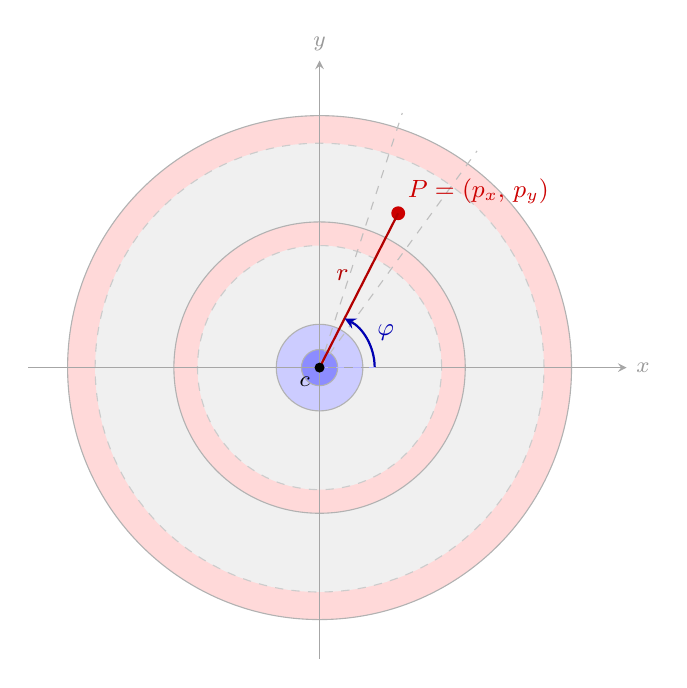
\begin{tikzpicture}[scale=1.0]

  % --- Zonenfüllungen ---
  \fill[gray!12] (0,0) circle (3.2cm);           % Single-Feld
  \fill[red!15]  (0,0) circle (3.2cm);
  \fill[gray!12] (0,0) circle (2.85cm);           % Zwischen Double und Triple
  \fill[red!15]  (0,0) circle (1.85cm);           % Triple-Ring (außen)
  \fill[gray!12] (0,0) circle (1.55cm);           % Single innen
  \fill[blue!20] (0,0) circle (0.55cm);           % Outer Bull
  \fill[blue!45] (0,0) circle (0.23cm);           % Bullseye

  % --- Kreislinien ---
  \draw[gray!60, thin]            (0,0) circle (3.20cm); % Double außen
  \draw[gray!40, thin, dashed]    (0,0) circle (2.85cm); % Double innen
  \draw[gray!60, thin]            (0,0) circle (1.85cm); % Triple außen
  \draw[gray!40, thin, dashed]    (0,0) circle (1.55cm); % Triple innen
  \draw[gray!60, thin]            (0,0) circle (0.55cm); % Outer Bull
  \draw[gray!60, thin]            (0,0) circle (0.23cm); % Bull

  % --- Beispielhafte Segmentlinien ---
  \draw[gray!50, thin, dashed] (0,0) -- (90:3.4cm);
  \draw[gray!50, thin, dashed] (0,0) -- (72:3.4cm);
  \draw[gray!50, thin, dashed] (0,0) -- (54:3.4cm);

  % --- Auftreffpunkt P ---
  % Winkel phi = 63°, Radius r = 2.2cm (Single-Feld)
  \coordinate (P) at (63:2.2cm);
  \fill[red!80!black] (P) circle (2.5pt);

  % --- Radiuslinie r ---
  \draw[red!70!black, thick] (0,0) -- (P)
      node[midway, above left, font=\small] {$r$};

  % --- Winkel-Bogen phi ---
  \draw[->, >=stealth, blue!70!black, thick]
      (0.7cm, 0) arc[start angle=0, end angle=63, radius=0.7cm];
  \node[blue!70!black, font=\small] at (28:0.95cm) {$\varphi$};

  % --- Koordinatenachsen ---
  \draw[->, >=stealth, gray!70, thin] (-3.7,0) -- (3.9,0)
      node[right, font=\footnotesize, gray!80] {$x$};
  \draw[->, >=stealth, gray!70, thin] (0,-3.7) -- (0,3.9)
      node[above, font=\footnotesize, gray!80] {$y$};

  % --- Hilfslinie: Horizontalprojektion (für phi) ---
  \draw[blue!30, thin, dashed] (0,0) -- (0.7cm, 0);

  % --- Punkt P Beschriftung ---
  \node[above right, font=\small, red!80!black] at (P) {$P = (p_x,\, p_y)$};

  % --- Mittelpunkt ---
  \fill (0,0) circle (1.8pt);
  \node[below left, font=\footnotesize] at (0,0) {$c$};

\end{tikzpicture}
\caption{Geometrische Grundlage der Score-Berechnung im normierten
Scheibenkoordinatensystem. Der Auftreffpunkt~$P$ wird durch den
Polarwinkel~$\varphi$ und den Radius~$r$ eindeutig einem Winkelsegment
sowie einer radialen Wertungszone zugeordnet.}
\label{fig:score_berechnung}
\end{figure}

\section{Evaluation}

Im Folgenden wird festgelegt, wie die in der Leitfrage formulierten Vergleichskriterien im Rahmen dieser Arbeit konkret gemessen werden.

\subsubsection{Erkennungsgenauigkeit}

Die Erkennungsgenauigkeit beider Ansätze wird anhand der mittleren IoU (mean IoU, mIoU) über alle Testbilder bewertet. Zusätzlich wird die Erkennungsrate als Anteil der Bilder ausgewiesen, bei denen ein IoU-Schwellwert von $\text{IoU} \geq 0{,}5$ erreicht wird \cite{everingham2010pascal}. Als Referenz dienen Binärmasken, die durch manuelle Annotation mithilfe des Polygon-Werkzeugs der Annotationsplattform \cite{roboflow2024} erstellt wurden und die Kontur der Dartscheibe näherungsweise beschreiben. Da beide Ansätze dieselbe nachgelagerte Segmentierungs- und Punktberechnungslogik verwenden, sind Unterschiede in der mIoU ausschließlich auf die jeweilige Lokalisierungsmethode zurückzuführen, was einen isolierten Vergleich beider Ansätze unter sonst identischen Bedingungen ermöglicht.

\subsubsection{Robustheit gegenüger Aufnahmebedingungen}

Zur Bewertung der Robustheit wird der Testdatensatz in Untergruppen eingeteilt, die jeweils eine spezifische Störbedingung repräsentieren. Untersucht werden Lichtverhältnisse (Über- und Unterbelichtung), Perspektivverzerrung (flache Aufnahmewinkel) sowie Skalierung (variierender Bildausschnitt). Die mIoU wird pro Untergruppe separat ausgewertet, um zu identifizieren, unter welchen Bedingungen die jeweilige Methode am stärksten beeinträchtigt wird \cite{szeliski_computer_2022}.

\subsubsection{Verarbeitungsgeschwindigkeit}

Die Verarbeitungsgeschwindigkeit wird als mittlere Inferenzzeit in Millisekunden pro Bild bestimmt und umfasst die vollständige Verarbeitungspipeline vom Eingabebild bis zur Erzeugung der resultierenden Maske. Die Experimente wurden auf einem Acer Aspire-13 Laptop mit einem Intel Core i5-1235U Prozessor der 12. Generation, 32 GB Arbeitsspeicher sowie dem Betriebssystem Windows-11 durchgeführt. 

Die Ausführung erfolgte CPU-basiert unter Verwendung von Python~3.11 und PyTorch~2.10. Zur Reduktion zufälliger Schwankungen wird für jedes Bild der Mittelwert über mindestens 50 Wiederholungen berechnet.

\subsubsection{Implementierungsaufwand}

Der Implementierungsaufwand wird qualitativ bewertet und umfasst den Aufwand zur Datenbeschaffung und -annotation, den Trainingsaufwand des U-Net-Modells sowie den Integrationsaufwand in eine mobile Anwendung. Da dieser Aspekt einer quantitativen Messung nicht zugänglich ist, wird er anhand einer strukturierten Beschreibung der jeweiligen Entwicklungsschritte dokumentiert und verglichen.